% !TEX root = ../lectures.tex
\section{Synchrotron Radiation}

Synchrotron radiation, denoted by the process \( e + B \rightarrow e + \gamma + B \), is emitted by relativistic charged particles as they undergo acceleration in a static magnetic field. In the non-relativistic regime, this is known as 
\textbf{cyclotron emission}.

Starting with the basic Larmor formula, the total power emitted by an accelerating or decelerating electron (or any charged particle) in c.g.s. units is:
%
\[
P = \frac{2}{3} q^2 \frac{a^2}{c^3}
\]
%
where \( a = \| \vb a \|\) is the acceleration.

The heuristic derivation of this formula includes: a) Radiative processes are proportional to \( q^2 \), as the cross-section \( \sigma \) is the square of the amplitude which for e.m. process is \( \propto q \), b) Consistency with relativity requires dependence only on acceleration, not velocity, since power is a relativistic invariant being the ratio of two time-like components, and c) Dimensional analysis justifies the \( a^2 \) term.

In relativistic scenarios, the Larmor formula is valid if \( a^2 \) is replaced by \( a^\mu a_\mu \), the invariant square of the four-acceleration. 

\begin{problem}
Demonstrate that \( a^\mu a_\mu \)  is a relativistic invariant.
\end{problem}

Considering the Lorentz force, the acceleration is perpendicular to velocity:
%
\[
\vb a = \frac{\vb F}{m} = \frac{\gamma q}{m} \left(\frac{\vb v}{c} \times \vb B \right)
\]
%
leading to:
%
\[
a^2 = \frac{q^2}{m^2} \frac{v_\perp^2}{c^2} \gamma^2 B^2 \longrightarrow a^2 = \frac{q^2}{m^2} \gamma^2 \beta^2 B^2 \sin^2 \theta
\]

The power emitted by synchrotron radiation in the limit \( \beta \rightarrow 1 \) is then:
%
\[
P_{\rm s} = \frac{2}{3} \frac{q^4 B^2}{m^2 c^3} \gamma^2 \sin^2 \theta
\]

Notably, synchrotron radiation is predominantly significant for leptons rather than nuclei, as \( P_{\rm s} \propto 1/m^4 \).

For an isotropic particle distribution, the average emitted power becomes:
%
\begin{remark}
\[
\langle P_{\rm s} \rangle = \frac{4}{9} \frac{q^4 B^2}{m^2 c^3} \gamma^2 = \frac{4}{3} c \sigma_{\rm T} \left(\frac{m_e}{m}\right)^2 \gamma^2 U_{\rm B}
\]
\end{remark}

using \( U_{\text{B}} = \frac{B^2}{8\pi} \) and \( \sigma_{\text{T}} = \frac{8\pi}{3} \left( \frac{q^2}{m_e c^2} \right)^2 \), and the average over the angle
%
\[
\langle \sin^2 \theta \rangle = \frac{1}{4\pi} \int d\Omega \sin^2 \theta = \frac{1}{4\pi} \int_0^{2\pi} \int_0^\pi \sin^2 \theta \sin \theta d\theta = \frac{2}{3}
\]

The electron energy loss timescale, important for understanding cooling rates, is:
%
\begin{remark}
\[
\tau_{\text{loss}} (\gamma) \simeq \frac{E}{| dE/dt |} = \frac{\gamma m_e c^2}{\langle P_s \rangle} = \frac{3}{4} \frac{m_e c}{\sigma_{\text{T}}} \frac{1}{\gamma U_{\text{B}}} \propto \frac{1}{E}
\]
\end{remark}
%
leading to the notable result that more energetic particles have shorter lifetimes.

\begin{problem}
The CRAB.
\end{problem}

To determine the emission spectrum of an electron with a specific energy, we consider the spectrum \( P_\nu \) as the frequency power spectrum of \( P(t) \), proportional to \( |a(t)|^2 \). To derive \( P_\nu \), we employ a Fourier transform, which translates the time-domain signal into its frequency components.

In synchrotron radiation, the effect of relativistic beaming is crucial. This phenomenon, combined with the fundamental gyromotion of electrons in a magnetic field, results in the emitted power being concentrated at frequencies much higher than the gyrofrequency \( \nu_g \) (see derivation in appendix).

Let's first derive the aberration formula, assuming the primed frame is seen from the unprimed frame as moving with speed $\beta = v/c$ along the x-axis:
%
\begin{eqnarray*}
c t^\prime & = & \gamma (c t - \beta x) \\
x^\prime & = & \gamma (x - \beta c t) \\
y^\prime & = & y 
\end{eqnarray*}

The velocity components transform as follows:
%
\begin{eqnarray*}
u_x & = & \frac{u'_x + \beta c}{1+\beta u'_x / c} \\
u_y & = & \frac{u'_y}{\gamma(1+\beta u'_x / c)} 
\end{eqnarray*}

Therefore, the emission angle \( \theta \) is given by:
%
\[
\tan \theta = \frac{u_y}{u_x} = \frac{u^\prime_y}{\gamma(u^\prime_x + \beta c)} = \frac{u^\prime \sin \theta^\prime}{\gamma(\beta c + u^\prime \cos \theta^\prime)} 
\]

For light (with \( u^\prime = c \)), the aberration formula becomes:
%
\begin{remark}
\[
\tan \theta = \frac{\sin \theta^\prime}{\gamma(\beta + \cos \theta^\prime)} 
\]
\end{remark}

\begin{figure}[t]
\centering
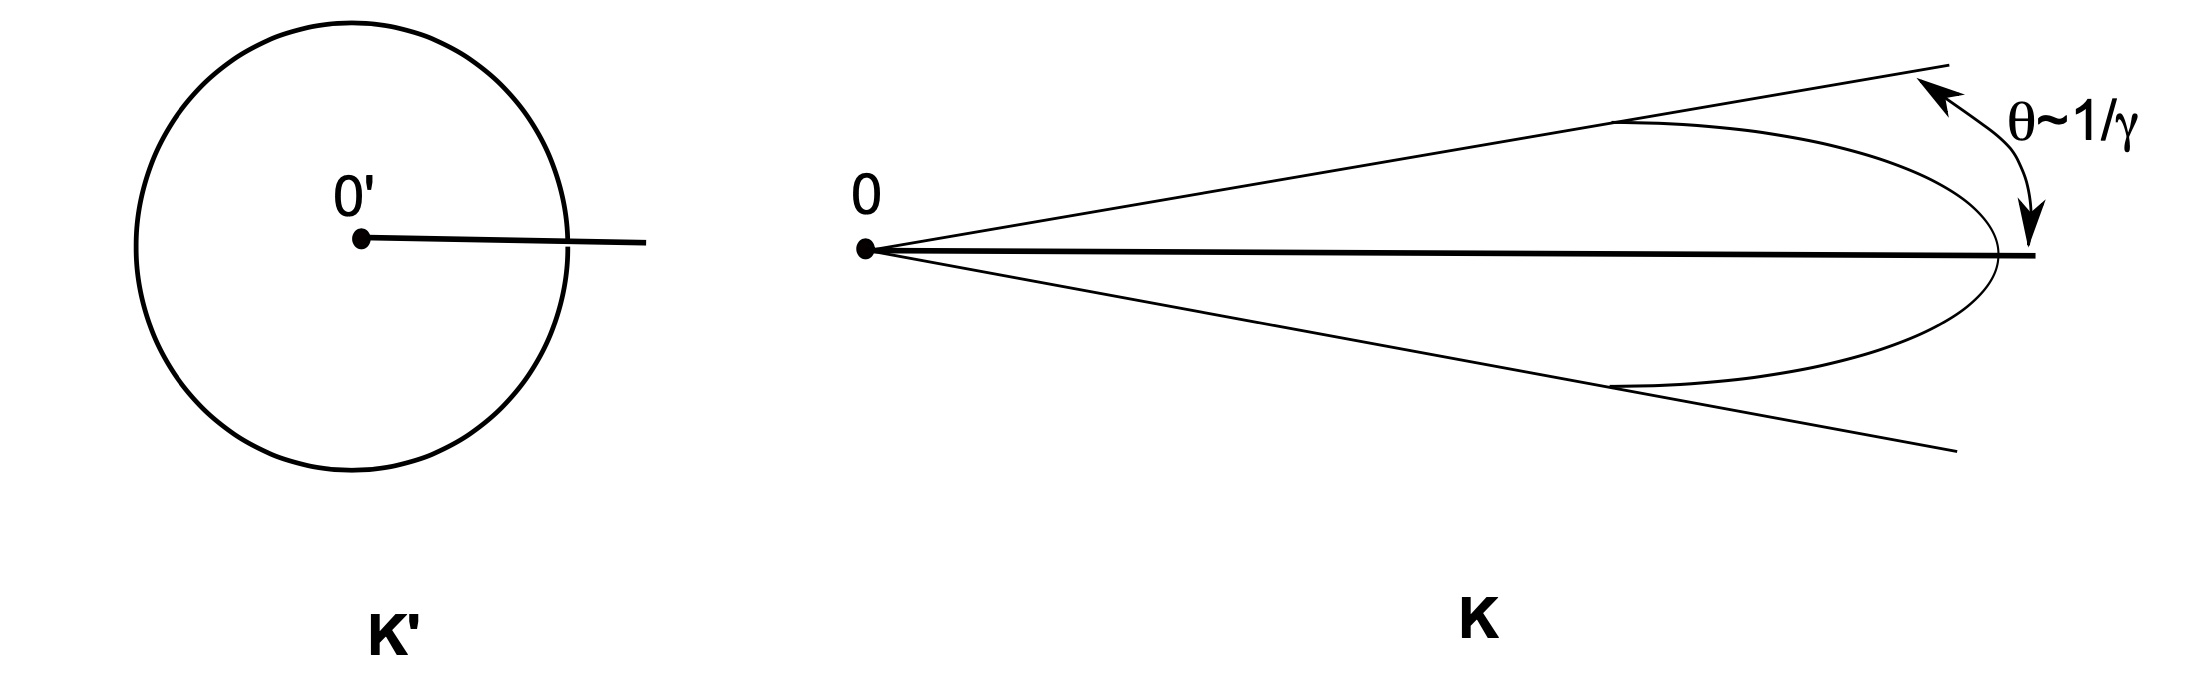
\includegraphics[width=0.8\textwidth]{aberration.jpg}
\caption{aberration}
\end{figure}

A photon emitted at \( \theta^\prime = 0 \) in the primed frame travels at \( \theta = 0 \) in the observer's frame. Conversely, a photon emitted at \( \theta^\prime = \frac{\pi}{2} \) travels at an angle \( \theta \) approximated by \( \theta \simeq \frac{1}{\gamma} \).

This indicates that emission isotropic at the source is not perceived as isotropic by an observer if there is a relativistic boost between them. This is particularly relevant for phenomena like gamma-ray bursts (GRBs), which are strongly beamed in the forward direction, forming a cone with an opening angle of approximately \( \sim \frac{2}{\gamma} \).

In the non-relativistic limit, the frequency of the emitted radiation corresponds to the gyro-frequency, leading to a mono-chromatic spectrum at this frequency.

However, in the relativistic regime, continuous emission is altered by the beaming effect. The signal is visible only at specific angles due to this effect. The resulting spectrum is still a Fourier transform of the time-dependent emission, but now it has a characteristic timescale \(  \Delta t \), giving a frequency spectrum peaked around \( \sim \frac{1}{\Delta t} \).

\begin{figure}[t]
\centering
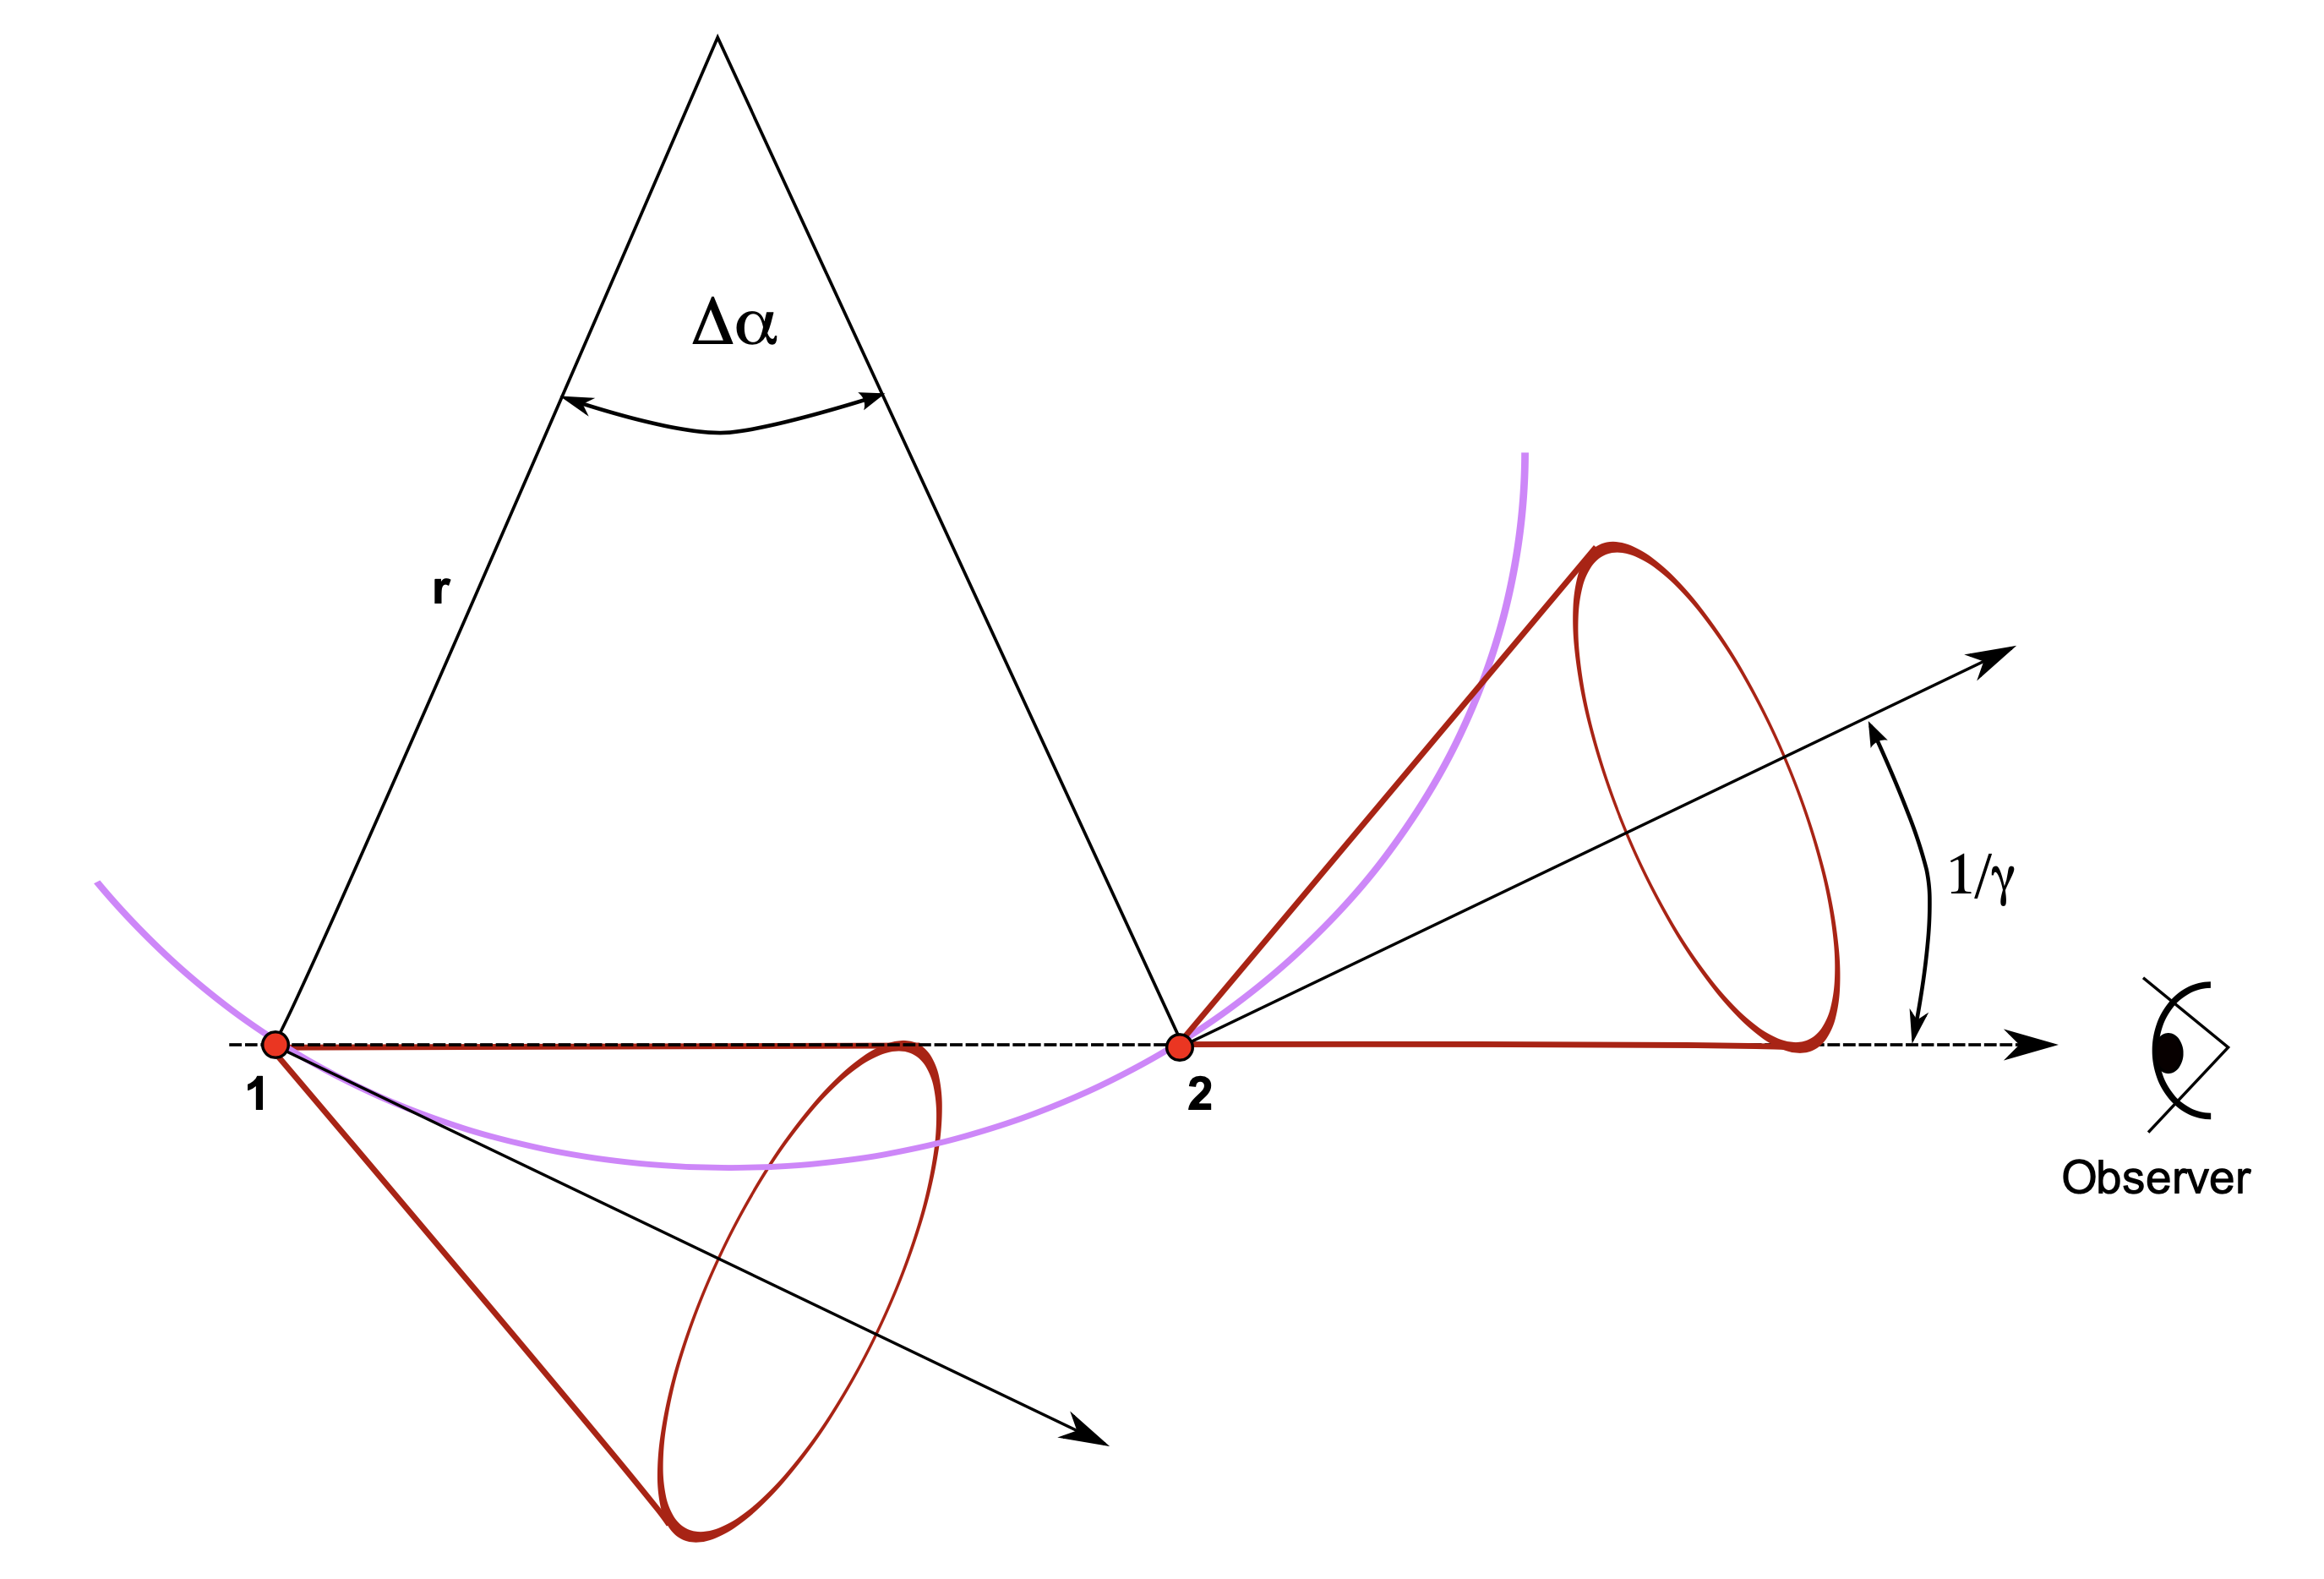
\includegraphics[width=0.8\textwidth]{opening.png}
\caption{opening}
\end{figure}

To determine the duration of emission as perceived by a distant observer, consider the time taken for an electron to move from point A to B. This segment of the trajectory corresponds to the period during which the radiation emitted by the electron falls within the observer's view because of the emitted cone:
%
\[
\Delta t = \frac{\text{AB}}{v}
\]

At the observer ($\delta t_i$ is the time for the \emph{photon} to reach the observer): 
%
\[
\Delta t_{\rm obs} = t_B + \delta t_B - (t_A  + \delta t_A) = (t_B - t_A) + (\delta t_B - \delta t_A) = \frac{\text{AB}}{v} - \frac{\text{AB}}{c} = \frac{\text{AB}}{v} (1-\beta)
\]

Using AB~$= \frac{2}{\gamma}r_{\rm L}$, we get:
%
\[
\Delta t_{\rm obs} = \frac{\text{AB}}{v} (1-\beta) \frac{1+\beta}{1+\beta} \overset{\beta \sim 1}{\simeq} \frac{\text{AB}}{v} \frac{1}{2\gamma^2} \simeq {\color{red}\frac{r_{\rm L}}{\gamma^3}}
\]

An observer sees a sequence of pulses of width:
%
\[
\Delta t_{\rm obs} \simeq \frac{1}{v \gamma^2 \nu_g} %\simeq \frac{1}{\gamma^3 \nu_L} 
\]

These pulses are separated by a gyration time 
%
\[
T \simeq \frac{1}{\nu_L} = \frac{\gamma}{\nu_g}
\]

\begin{figure}[t]
\centering
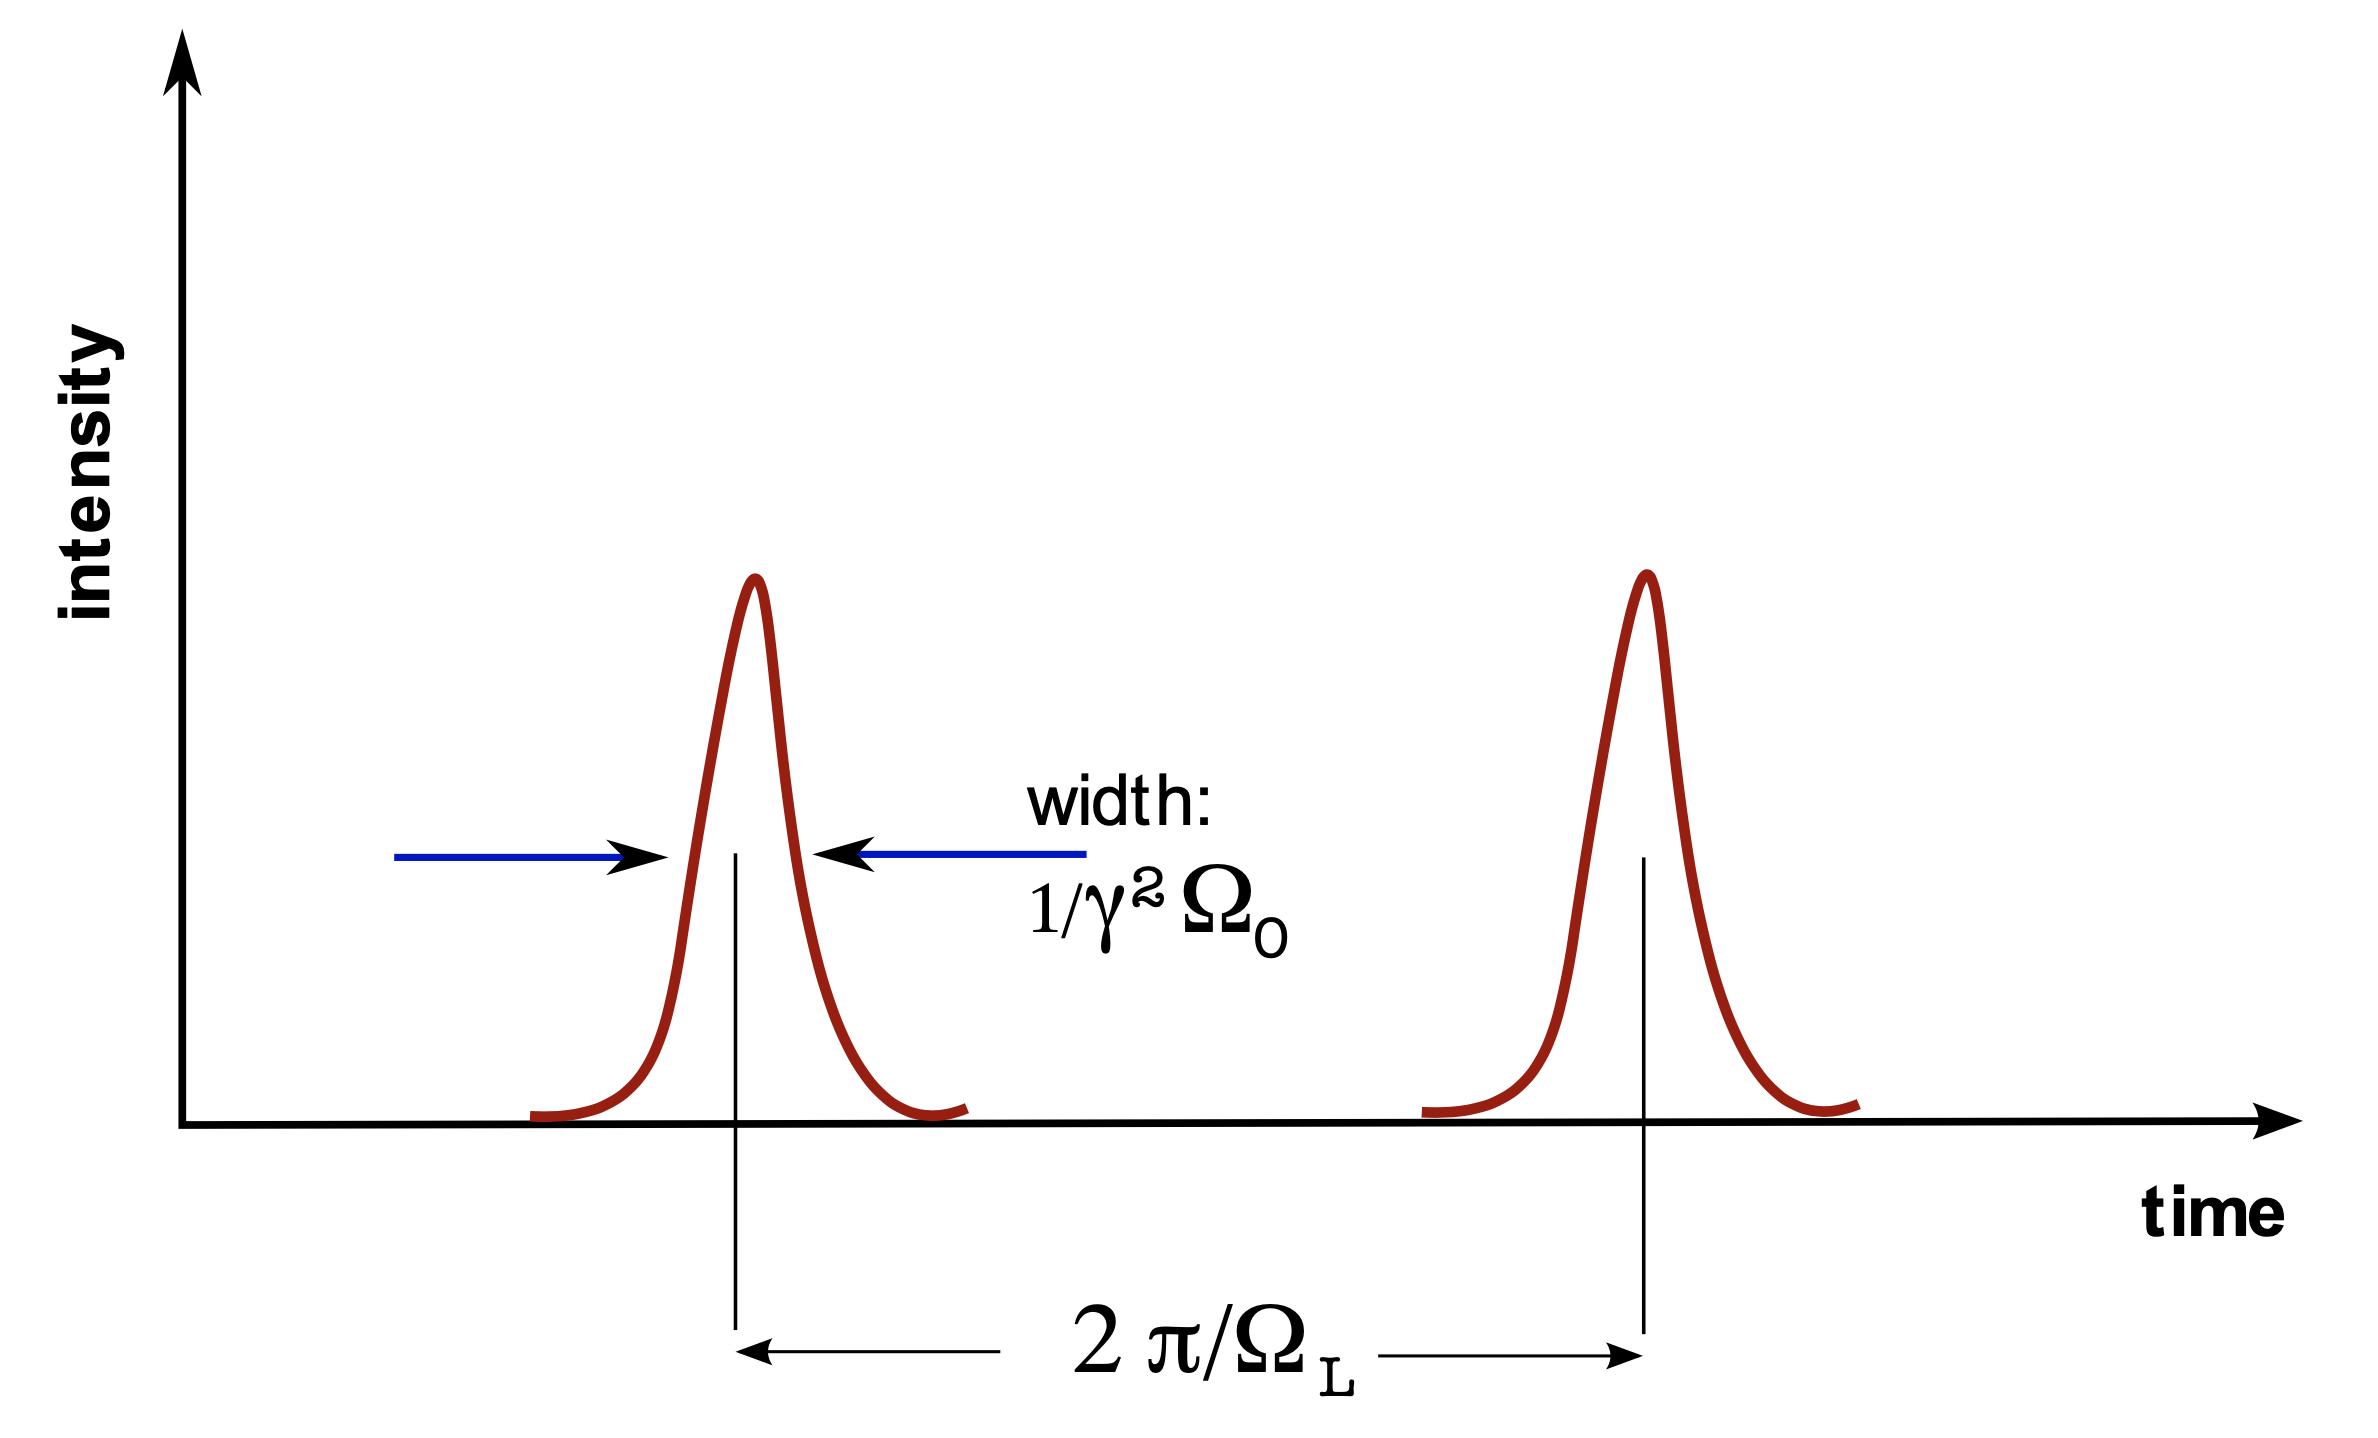
\includegraphics[width=0.8\textwidth]{observedelectricfield.png}
\caption{observedelectricfield}
\end{figure}

Thus, in the relativistic limit, the spectrum experiences a \( \gamma^2 \) boost compared to the cyclotron frequency:
%
\begin{remark}
\[
\nu_s \sim \frac{1}{\Delta t_{\rm obs}} = \frac{\gamma^3}{r_{\rm L}} = \gamma^2 \nu_g
\]
\end{remark}

\begin{problem}
Compute the properties of the Galactic radio emission.
\end{problem}

The full result for a single electron with Lorentz factor \( \gamma \) is:
%
\[
P_\nu(\nu, \gamma, \theta) = \frac{\sqrt 3 q^3 B}{m_e c^2} \sin \theta F\left(\frac{\nu}{\nu_c}\right)
\]
%
where $P_\nu$ is the power per \emph{unit of frequency}, the characteristic frequency $\nu_c = \frac{3}{4\pi} \gamma^2 \frac{qB}{m_e c} \sin \theta$, and the synchrotron function is
%
\[
F(x) = x \int_x^\infty K_{5/3} (x^\prime) dx^\prime
\]

A useful approximation for \( P_\nu \) is 
%
\[
P_\nu \simeq 1.8 \left(\frac{\nu}{\nu_c}\right)^{1/3} \exp\left(-\frac{\nu}{\nu_c}\right)
\]
%
notice that the \emph{peak} frequency is approximately  \( \nu_{\rm max} \simeq 0.29 \nu_c \).

\subsection{Quantum correction}

In our previous analysis of synchrotron radiation, we assumed that the motion of electrons does not change significantly due to photon emission. However, considering that photons carry momentum, there should be some recoil effect on the emitting electron. This aspect becomes particularly relevant when the energy of the emitted synchrotron photon, \( h \nu_s \), approaches the electron's relativistic energy, \( \gamma m_e c^2 \). Given that \( \nu_s \propto \gamma^2 \), this effect is more pronounced at higher energies.

To quantify this, we introduce the parameter \( \chi \):
%
\[
\chi = \frac{B}{B_q}\frac{p}{mc} \sim \frac{h\nu_s}{\gamma mc^2}
\]

Here, \( p \) is the electron momentum, and \( B_q = \frac{m^2 c^3}{e \hbar} \approx 4.4 \times 10^{13} \) G is a characteristic magnetic field strength.

For \( \chi \ll 1 \), the motion can be considered Newtonian, while for \( \chi \gg 1 \), quantum effects dominate. In extremely strong magnetic fields, like those found in pulsar atmospheres (\( \sim 10^{15} \) G), quantum effects become significant even for relatively low electron momenta.

According to Landau, the power radiated in the quantum regime (\( \chi \gg 1 \)) is:
%
\[
P_q \propto \frac{e^2 m^2 c^3}{\hbar^2} \left( \frac{B}{B_q}\right)^{2/3} \gamma^{2/3}
\]

This indicates that the power dependency shifts from \( \gamma^2 \) to \( \gamma^{2/3} \) in the quantum regime.

The spectrum in this regime peaks broadly and almost flatly around a frequency that satisfies:
%
\[
\frac{h\nu}{E - h\nu} \sim \chi
\]

For \( \chi \ll 1 \), the emitted frequency \( \nu \) is approximately equal to the synchrotron frequency \( \nu_s \). In contrast, for \( \chi \gg 1 \), \( h\nu \) is comparable to the initial energy \( E \), indicating that the emitted photon carries away a significant portion of the electron's energy. This results in catastrophic energy losses and a non-continuous process, necessitating a \emph{Monte Carlo} approach for accurate modeling.

\subsection{Synchrotron emission by an electron population}

Assume to have a population of electrons with a power-law distribution in energy within some given range:
%
\[
n(\gamma) d\gamma = n_0 \gamma^{-p} d\gamma \quad \gamma_{\rm min} < \gamma < \gamma_{\rm max} 
\]	
%
where $n(\gamma) d\gamma$ is the electron volume density, and usually the slope is $p \sim 2-3$.

The specific emissivity is given by
%
\begin{equation*}
j_\nu = \int_1^\infty \langle P_\nu(\gamma) \rangle n(\gamma) d\gamma
\end{equation*}
%
where $P_\nu$ is the power emitted per unit frequency.

We simplify our calculations assuming a $\delta$-function for $P_\nu$:
%
\begin{equation*}
P_\nu(\gamma) \simeq \langle P_s \rangle \delta(\nu - \nu_c)
\end{equation*}
%
follows
%
\begin{equation*}
j_\nu = \frac{4}{3} c \sigma_{\rm T} U_{\rm B} n_0 \int_{\gamma_{\rm min}}^{\gamma_{\rm max}} \gamma^{2-p} \delta(\nu - \gamma^2 \nu_{\rm L}) d\gamma
\end{equation*}
%
finally
%
\begin{remark}
\[ 
j_\nu = \frac{2}{3} c \sigma_{\rm T} n_0 \frac{U_{\rm B}}{\nu_{\rm L}} \left( \frac{\nu}{\nu_{\rm L}} \right)^{\color{red}-\frac{p-1}{2}}
\]
\end{remark}
%
which is valid in the range $\gamma^2_{\rm min} \nu_{\rm L} < \nu < \gamma^2_{\rm max} \nu_{\rm L}$

%\begin{center}
%\includegraphics[scale=0.18]{figures/synchropowerlaw.png}
%\end{center}

Outside the validity limits we have to use the complete expression and we obtain 
%
\begin{equation*}
j_\nu \propto \nu^{1/3} \quad\text{ for }\quad \nu < \nu_{\rm min}
\end{equation*}
%
and
%
\begin{equation*}
j_\nu \propto \exp \left(-\frac{\nu}{\nu_{\rm max}}\right) \quad\text{ for }\quad \nu > \nu_{\rm max}
\end{equation*}

\subsection{Kinetic equation for electron evolution}

TO BE DONE

\subsection{Synchrotron Self-Absorption}

The Synchrotron self-absorption corresponds to the inverse process where a free electron can absorb a synchrotron photon in a magnetic field $e+B+\gamma\rightarrow e+B$.

We provide here an heuristic derivation of how this process impacts on the spectrum. In fact, we have a population of electrons which are emitting radiation and absorbing radiation and we want to compute the intensity using the radiative transfer equation.

Let's remind that for a thermal distribution of electrons, the source function would correspond to the black-body
%
\[
S_\nu = {\color{red}\left(\frac{2\nu^2}{c^2}\right)} {\color{blue}\left(\frac{h\nu}{\exp(h\nu / kT) - 1}\right)} 
\propto {\color{red}\nu^2} {\color{blue}\langle E \rangle}
\]
%
where the first term is the \emph{phase-space factor} and the second is the \emph{mean electron energy} emitting photons at frequency $\nu$.

In fact, in the Rayleigh-Jeans limit $kT \gg h\nu$ and
%
\[
\langle E \rangle \simeq kT \lim_{x\rightarrow 0} \frac{x}{\exp x - 1} \sim kT
\]

For a non-thermal synchrotron radiation $kT$ must be replaced by the mean energy of an electron emitting synchrotron radiation at frequency $\nu$
%
\begin{equation*}
\nu \simeq \gamma^2 \nu_{\rm L} \rightarrow \gamma \sim \left(\frac{\nu}{\nu_{\rm L}}\right)^{1/2}
\end{equation*}
%
follows
%
\begin{equation*}
S_\nu \sim \left( \frac{2\nu^2}{c^2} \right) \gamma m_e c^2
\propto \left( \frac{2\nu^2}{c^2} \right) \left(\frac{\nu}{\nu_{\rm L}}\right)^{1/2} 
\propto B^{-1/2} \nu^{5/2} 
\end{equation*}

%\begin{center}
%\includegraphics[scale=0.06]{figures/x299.png}
%\end{center}

From the definition of the source term \( S_\nu = \frac{j_\nu}{\alpha_\nu} \), follows
%
\[
\alpha_\nu = \frac{j_\nu}{S_\nu} 
\propto (B^{\frac{p+1}{2}} \nu^{-\frac{p-1}{2}}) (B^{\frac 1 2} \nu^{-\frac 5 2})
= B^{\frac{p+2}{2}} \nu^{-\frac{p + 4}{2}}
\]

We notice that $\alpha_\nu$ decreases towards higher frequencies, so it will be relevant at low energies.

From the transfer equation $I_\nu = S_\nu [1 - \exp(-\tau_\nu)]$ and reminding $\tau_\nu = \alpha_\nu s$, we identify the following limiting regimes:
%
\begin{itemize}
\item for $\tau_\nu \gg 1$ corresponding to small frequencies $I_\nu \rightarrow S_\nu$

\item for $\tau_\nu \ll 1$ corresponding to large frequencies $I_\nu \rightarrow S_\nu \alpha_\nu s = j_\nu s$
\end{itemize}

Therefore for each source exists a frequency $\nu_B$ where $\tau_B = 1$ and the corresponding spectrum will be:
%
\begin{itemize}
\item for $\nu \ll \nu_B$ (optically thick) and $I_\nu \propto \nu^{5/2}$, notice independent on $p$!

\item for $\nu \gg \nu_B$ (optically thin) and $I_\nu \propto \nu^{-\frac{p-1}{2}}$
\end{itemize}

% TYPICAL SPECTRUM OF A RADIO SOURCE

\begin{problem} Estimate the age of the source from the break.
\end{problem}

%As our observing frequency increases, we see photons coming from regions of the source that are progressively deeper and deeper, and as we do so the total flux density increases. However, of course, eventually we reach a point where we can “see all the way through” the plasma, and above this frequency we recover the underlying power-law distribution.

%\begin{center}
%\includegraphics[scale=0.14]{figures/selfabsorption.png}
%\end{center}

%Representative spectra of \textbf{radio galaxies and quasars}. The radio source 3C 84 in the nearby galaxy NGC 1275 contains a very compact nuclear component that is opaque below about 20 GHz. The radio galaxy 3C 123 is transparent at all plotted frequencies, and energy losses steepen its spectrum above a few GHz. The quasar 3C 48 is synchrotron self-absorbed only below 100 MHz, while the quasar 3C 454.3 contains structures of different sizes that become opaque at different frequencies.

\subsection{Minimum Energy and Equipartition}

The existence of a synchrotron source implies the presence of relativistic electrons with some energy density $U_{\rm e}$ and a magnetic field whose energy density is $U_{\rm B} = \frac{B^2}{8\pi}$. 
%
What is the \emph{minimum total energy in relativistic particles and magnetic fields} required to produce a synchrotron source of a given radio luminosity?

The energy density in particles is
%
\[
U_e = \int_{\gamma_{\rm min}}^{\gamma_{\rm max}} E n(\gamma) d\gamma
%\simeq n_0 m_e c^2 \int_{\gamma_{\rm min}}^{\infty} \gamma^{1-p} d\gamma n_0 m_e c^2 = \frac{n_0 m_e c^2}{p-2} \gamma_{\rm min}^{-(p-2)}
\]
%
and the corresponding luminosity is
%
\[
\mathcal L = V \int_{\gamma_{\rm min}}^{\gamma_{\rm max}} \left| \frac{dE}{dt} \right| n(\gamma) d\gamma
%\simeq n_0 m_e c^2 \int_{\gamma_{\rm min}}^{\infty} \gamma^{1-p} d\gamma n_0 m_e c^2 = \frac{n_0 m_e c^2}{p-2} \gamma_{\rm min}^{-(p-2)}
\]

For a power-law distribution $n(\gamma) \propto \gamma^{-p}$, and using $P \propto \gamma^2 U_B$ the ratio between the two is proportional to
%
\begin{equation*}
\frac{U_e}{\mathcal L} \propto \frac{1}{U_B} \frac{\int_{\gamma_{\rm min}}^{\gamma_{\rm max}} \left( \frac{\gamma}{\gamma_{\rm min}}\right)^{1-p} d\gamma}{\int_{\gamma_{\rm min}}^{\gamma_{\rm max}}  \left( \frac{\gamma}{\gamma_{\rm min}}\right)^{2-p}  d\gamma} \propto \frac{1}{U_B} \frac{\gamma_{\rm min}^{2-p}}{\gamma_{\rm min}^{3-p}} \propto \frac{1}{U_B \gamma_{\rm min}}
\end{equation*}	

Finally, $\nu_s \propto \gamma^2 B$ therefore $\gamma \propto B^{-1/2}$, for a fixed frequency, and thereby $U_e / \mathcal L \propto B^{-3/2}$.  

We conclude that the electron energy density needed to produce a given synchrotron luminosity scales as $U_e \propto B^{-3/2}$. % while the magnetic energy density $U_B \propto B^2$.

The minimum of the total energy density $U$ as a function of $B$ occurs at
%
\begin{equation*}
\frac{dU}{dB} = \frac{d}{dB} (U_e + U_B) = 0 \rightarrow \frac{-3/2}{B} U_e + \frac{2}{B} U_B = 0
\end{equation*}

The ratio of cosmic-ray particle energy density to magnetic field energy that minimizes the total energy is
%
\begin{remark}
\[
\frac{U_e}{U_B} = \frac{4}{3}
\]
\end{remark}

This ratio is nearly unity, so minimum energy constraint for an optically thin synchrotron source places similar amount of energy in particles as in magnetic fields (equipartition).

\begin{problem}
Cygnus A (3C 405)
\end{problem}

%Physical motivated.